\chapter{Validación de la solución}
\label{chap:pruebas}

\section{Metodología de la validación}
El objetivo principal de la validación es asegurar que la solución desarrollada, \textit{PhenoScore}, cumpla con los requisitos funcionales definidos y sea aceptada por los usuarios finales como una herramienta útil, eficiente y fácil de usar para el análisis de \textit{Polygenic Risk Scores} (PRS).
Para ello, se ha diseñado un enfoque de validación integral basado en tres dimensiones complementarias:

\begin{enumerate}
    \item Validación funcional: Se verifica que las funcionalidades principales de la herramienta operan correctamente, permitiendo a los usuarios realizar las tareas clave sin errores críticos.
    \item Validación de usabilidad: Se evalúa la facilidad de uso y la satisfacción de los usuarios mediante la observación directa y la aplicación de cuestionarios específicos.
    \item Validación de aceptación tecnológica: Se mide la intención de uso y la aceptación de \textit{PhenoScore} por parte de los usuarios utilizando el modelo de aceptación tecnológica (\textit{Technology Acceptance Model, TAM})\cite{davis1989}.
\end{enumerate}

Para estructurar esta validación, se establecen tres capas o niveles de análisis:

\begin{enumerate}
    \item \textit{User Stories}: Se evalúa si los usuarios pueden completar las tareas definidas en las historias de usuario, proporcionando una validación desde la perspectiva del usuario.
    \item Requisitos no funcionales: Se realiza una medición técnica directa de aspectos como rendimiento, seguridad y tiempos de respuesta para comprobar el cumplimiento de los requisitos no funcionales establecidos.
    \item Modelo \textit{TAM}: Se aplica un cuestionario basado en una escala \textit{Likert} para evaluar la percepción de utilidad, facilidad de uso e intención de uso futuro.
\end{enumerate}


\subsection{Participantes}

La validación de \textit{PhenoScore} se lleva a cabo con la participación de un grupo reducido pero representativo de usuarios que reflejan los diferentes perfiles de los \textit{stakeholders} involucrados en el uso y desarrollo de la herramienta. Estos usuarios realizan una serie de tareas guiadas y responden a cuestionarios que permiten obtener datos cualitativos y cuantitativos para el análisis de los resultados.

Los usuarios seleccionados para la validación son los siguientes:

\begin{itemize}
    \item \textbf{Perfil 1: Investigador Experto en Genética (Usuario Final Científico).} Un investigador con profundos conocimientos en el análisis de Puntuaciones de Riesgo Poligénico (PRS) y biología. Este perfil, familiarizado con las herramientas científicas existentes, es ideal para evaluar la adecuación funcional y la integración tecnológica de la plataforma en un contexto de investigación real.
    
    \item \textbf{Perfil 2: Ingeniero de Software Experto (Usuario Técnico).} Un experto en informática con amplia experiencia en el desarrollo de software, pero con conocimientos limitados en biología y análisis genéticos. Su participación aporta una perspectiva técnica crítica, centrada en evaluar la usabilidad desde un punto de vista informático, la robustez del sistema y la calidad de la implementación.

    \item \textbf{Perfil 3: Biólogo No Técnico (Usuario Final Objetivo).} Un profesional con formación y experiencia en biología y genética, pero con un conocimiento limitado en informática y aspectos técnicos de software. Este perfil representa al grupo de usuarios finales objetivo de la plataforma. Su participación es esencial para evaluar la facilidad de uso, la accesibilidad y la adecuación de la interfaz para un usuario no experto en el dominio técnico.

\end{itemize}

La selección de estos perfiles permite cubrir las distintas dimensiones de validación, asegurando una evaluación equilibrada desde los puntos de vista científico, técnico y de usuario final.

\subsection{Procedimiento}

El procedimiento de validación ha sido diseñado para ser completado en una única sesión por cada participante, con una duración aproximada de 30-45 minutos, y ha sido estructurado en dos fases principales:

\begin{enumerate}
    \item Sesión de prueba guiada (25-35 minutos):
    \begin{enumerate}
    \item Introducción (5 min): Se realiza una breve presentación de \textit{PhenoScore}, explicando sus objetivos y funcionalidades principales.
    \item Realización de Tareas (20-30 min): Se solicita a cada participante que realice una serie de tareas representativas, diseñadas a partir de las \textit{user stories} principales (iniciar sesión, crear un análisis, configurar parámetros, ejecutarlo y visualizar resultados). Durante este proceso, un investigador observa directamente la interacción del usuario con la plataforma, tomando notas sobre el tiempo, los errores y la facilidad para completar cada tarea.
    \end{enumerate}
    \item Cuestionarios post-prueba (5-10 minutos):
    Al finalizar la sesión práctica, se pide a los participantes que completen un cuestionario basado en el Modelo de Aceptación Tecnológica (\textit{TAM}), con el fin de recoger su percepción subjetiva sobre la herramienta.
\end{enumerate}


\subsection{Instrumentos de medición}
%(En los instrumentos de medición podrías dar 1 poco más de detalle de qué se espera que hagan en cada user story y cómo se les indica a los testers que realicen esas tareas)

Para recoger los datos de manera estructurada se han diseñado tres instrumentos de medición principales, cada uno enfocado en una dimensión diferente de la evaluación de la plataforma.

\subsubsection{Guión de tareas guiadas (validación funcional)}

Para evaluar la funcionalidad principal y la usabilidad de la plataforma, se ha preparado un guion de tareas basado en las historias de usuario más relevantes. Durante la sesión de validación, se le ha pedido a cada participante que complete estas tareas en secuencia, mientras un observador toma notas sobre el proceso. A cada participante se le ha proporcionado un contexto inicial y se le ha guiado a través de los siguientes escenarios:

\renewcommand{\arraystretch}{1.8} % Un valor intermedio para que no quede tan espaciado
\begin{table}[H]
    \centering
    \small
    \begin{tabularx}{\textwidth}{XX}
        \toprule
        \textbf{Tarea (HU Asociada)} & \textbf{Descripción del Escenario y Pasos a Realizar} \\
         \toprule
        \textbf{HU01: Iniciar Sesión} & 
        \textbf{Objetivo:} Acceder a la plataforma de forma segura. \newline
        \textbf{Pasos: }\textit{Inicie sesión en la aplicación utilizando las credenciales proporcionadas para acceder a su espacio de trabajo personal.} \\

        \textbf{HU02 y HU04: Explorar y Gestionar el Panel} & 
        \textbf{Objetivo:} Familiarizarse con la interfaz principal, localizar y gestionar un análisis existente. \newline
        \textbf{Pasos: }\textit{Una vez dentro, explore el panel de control. Localice un análisis y usando los botones de acción, compruebe su configuración y, posteriormente, elimínelo.} \\

        \textbf{HU03, HU05-07: Crear y Configurar un Análisis} & 
        \textbf{Objetivo:} Completar el flujo de creación de un nuevo análisis desde cero. \newline
        \textbf{Pasos: }\textit{A continuación, cree un nuevo análisis. Asígnele un nombre, suba el fichero genómico correspondiente, seleccione dos modelos PRS de su elección y configure el umbral de ancestría."} \\

        \textbf{HU08: Ejecutar el Análisis} & 
        \textbf{Objetivo:} Iniciar el procesamiento del análisis configurado. \newline
        \textbf{Pasos: }\textit{Una vez configurado, inicie la ejecución del análisis. Verifique que el nuevo análisis aparece en el panel de control con el estado \textit{running}.} \\

        \textbf{HU09 y HU10: Visualizar y Exportar Resultados} & 
        \textbf{Objetivo:} Acceder al informe de un análisis completado y exportarlo. \newline
        \textbf{Pasos: }\textit{Por último, localice un análisis previamente completado, acceda a su informe de resultados y utilice la opción para exportarlo."} \\
        \bottomrule
    \end{tabularx}
    \caption{Guion de tareas guiadas para la validación funcional.}
    \label{tab:validacion-funcional}
\end{table}

El criterio de éxito para cada tarea ha sido su finalización exitosa por parte del usuario, sin errores críticos y en un tiempo considerado razonable. La medición se ha realizado mediante observación directa, registrando una variable binaria ( \cmark\ Cumplida / \xmark\ No cumplida) y anotando cualitativamente cualquier dificultad o comentario expresado por el participante.

\subsubsection{Requisitos no funcionales (RNF):}
La validación de los RNF se ha realizado mediante una combinación de inspección técnica, pruebas específicas y el uso de herramientas automatizadas:

\renewcommand{\arraystretch}{1.3} % más espacio entre filas
\begin{table}[H]
    \centering
    \small
    \begin{tabularx}{1\textwidth}{cX}
        \toprule
        \textbf{Requisito} & \textbf{Comprobación} \\
        \midrule
        RNF-001 (Seguridad) & Verificación de la correcta implementación de \textit{Auth0} y la presencia del cifrado \textit{HTTPS} \\
        RNF-002 (Tiempo de carga) & Medición directa del tiempo de carga del panel de control principal usando las herramientas de desarrollo del navegador \\
        RNF-003 (\textit{Lighthouse}) & Ejecución de una auditoría \textit{Lighthouse} sobre la aplicación desplegada para obtener métricas de rendimiento y buenas prácticas \\
        RNF-004 (Interfaz intuitiva) & La plataforma debe ser percibida como fácil de usar por los usuarios y llevar a cabo las tareas sin errores.\\

        \bottomrule
    \end{tabularx}
    \caption{Comprobación de requisitos no funcionales}
    \label{tab:validacion-RNF}
\end{table}


\subsubsection{Modelo de aceptación tecnológica (TAM):}
Se ha utilizado un cuestionario con ítems formulados en una escala \textit{Likert} de 5 puntos (de 1: Totalmente en desacuerdo, a 5: Totalmente de acuerdo). El cuestionario se ha dividido en las tres dimensiones clásicas del modelo:

\renewcommand{\arraystretch}{1.3} % más espacio entre filas
\begin{table}[H]
    \centering
    \small
    \begin{tabularx}{1\textwidth}{lX} 
        \toprule
        \textbf{Elemento} & \textbf{Ítem} \\
        \toprule
        \multicolumn{2}{l}{\textbf{PEOU (Facilidad de Uso Percibida)}} \\ \midrule
        PEOU1 & Creo que es fácil configurar y ejecutar análisis de PRS en la plataforma. \\
        PEOU2 & Me resultó fácil cargar y gestionar archivos genómicos (\textit{VCF}, \textit{PLINK}, etc.). \\
        PEOU3 & Creo que la información mostrada sobre modelos PRS y poblaciones de referencia es adecuada y suficiente. \\
        PEOU4 & Pienso que la forma en que se visualizan los resultados de PRS es útil y comprensible. \\
        PEOU5 & En general, encontré \textit{PhenoScore} intuitiva y fácil de usar. \\
        \bottomrule
        \multicolumn{2}{l}{\textbf{PU (Utilidad Percibida)}} \\ \midrule
        PU1 & Creo que los resultados de análisis PRS mostrados son claros y útiles para mi trabajo. \\
        PU2 & Creo que \textit{PhenoScore} reduciría el tiempo y esfuerzo requerido para realizar análisis PRS. \\
        PU3 & Creo que \textit{PhenoScore} ofrece una solución efectiva para ejecutar análisis de riesgo poligénico. \\
        PU4 & Creo que \textit{PhenoScore} mejora mi capacidad para gestionar y organizar análisis genómicos. \\
        PU5 & En general, pienso que \textit{PhenoScore} es una herramienta útil para mi práctica profesional. \\
        \bottomrule
        \multicolumn{2}{l}{\textbf{ITU (Intención de Uso)}} \\ \midrule
        ITU1 & Tengo intención de usar \textit{PhenoScore} regularmente en mi trabajo futuro. \\
        ITU2 & Recomendaría \textit{PhenoScore} a mis colegas para realizar análisis PRS. \\
        \bottomrule
    \end{tabularx}
    \caption{Ítems de validación TAM (PEOU, PU e ITU).}
    \label{tab:tam-items}
\end{table}
\renewcommand{\arraystretch}{1.0} % Restaurar el valor por defecto



\section{Resultados}
A continuación, se presentan los resultados obtenidos de la sesión de validación, organizados según las tres capas metodológicas definidas.
\begin{itemize}
    \item \textbf{Validación funcional:} Verificación de que las funcionalidades principales funcionan correctamente
    \item \textbf{Validación de usabilidad:} Evaluación de la facilidad de uso y satisfacción del usuario
    \item \textbf{Validación no funcional:} Medición directa de requisitos de rendimiento, seguridad y escalabilidad
    \item \textbf{Validación de aceptación tecnológica:} Medición de la intención de uso mediante el modelo \textit{TAM}
\end{itemize}

\subsection{Validación funcional y de usabilidad}

La validación funcional se ha evaluado mediante la observación directa de los participantes mientras ejecutan el guion de tareas guiadas (descrito en la Tabla~\ref{tab:validacion-funcional}). El objetivo es verificar si las funcionalidades principales operan correctamente y si los usuarios pueden completar las tareas clave de forma autónoma.

\textbf{Resultados de la Ejecución de Tareas}

Los tres participantes han sido capaces de completar con éxito el 100\% de las tareas propuestas en el guion. No se han registrado errores críticos que hayan impedido la finalización de ninguno de los flujos de trabajo principales, desde el inicio de sesión hasta la creación, ejecución y visualización de resultados de un análisis.

\textbf{Observaciones Cualitativas de Usabilidad}

Además de la tasa de éxito, se han registrado observaciones cualitativas y los tiempos de ejecución, que sirven como un indicador indirecto de la facilidad de uso y la curva de aprendizaje de la plataforma para cada perfil de usuario. Los tiempos totales para completar el guion completo han sido:
\begin{itemize}
\item \textbf{Perfil 1} (Investigador Experto en Genética): 18 minutos.
\item \textbf{Perfil 2} (Ingeniero de Software Experto): 10 minutos.
\item \textbf{Perfil 3} (Biólogo No Técnico - Usuario Objetivo): 23 minutos.
\end{itemize}

\textbf{Análisis de los Resultados de Usabilidad}

Los resultados son consistentes con las expectativas. El Perfil 2 (Ingeniero), con alta familiaridad en el uso de aplicaciones web complejas, ha completado las tareas en el menor tiempo, lo que sugiere que la interfaz sigue patrones de diseño intuitivos para un usuario técnico.

El Perfil 1 (Investigador en Genética), aunque experto en el dominio del problema, ha tardado un tiempo intermedio, probablemente debido a la fase de adaptación a una nueva herramienta y a una exploración más detallada de las opciones bioinformáticas.

Es de especial interés el resultado del Perfil 3 (Usuario Objetivo). A pesar de ser el perfil con menor conocimiento técnico, ha sido capaz de completar todas las tareas de forma autónoma en un tiempo muy razonable (23 minutos). Esto constituye una evidencia sólida de que la plataforma cumple su principal objetivo de reducir la barrera tecnológica y ser accesible para usuarios no expertos en informática. Aunque su tiempo ha sido el más elevado, el éxito en la finalización de las tareas indica que la interfaz es lo suficientemente clara para este perfil.

En conclusión, la validación funcional ha sido exitosa, demostrando que la plataforma es robusta y cumple con los requisitos definidos en las historias de usuario.

\subsection{Validación de requisitos no funcionales}

La evaluación de los RNF se ha centrado en aspectos de rendimiento y seguridad, mediante mediciones directas y el uso de herramientas automatizadas.
\begin{itemize}
    \item \textbf{RNF-001 (Seguridad):} Se ha verificado mediante inspección que toda la comunicación con el servidor se realiza a través de \textit{HTTPS}, garantizando el cifrado de los datos. La integración con \textit{Auth0} delega la gestión de credenciales a un proveedor especializado, cumpliendo con los estándares de seguridad. \textbf{Resultado:} Cumplido.
    \item \textbf{RNF-002 (Tiempo de Carga):} Utilizando las herramientas de desarrollo del navegador, se ha medido el tiempo de carga del panel de control principal. El tiempo promedio de carga completa del \textit{DOM} ha sido de 1.8 segundos en una conexión de red estándar, cumpliendo el requisito de ser inferior a 2 segundos. \textbf{Resultado:} Cumplido.
    \item \textbf{RNF-003(Rendimiento General- \textit{Lighthouse}):} La evaluación de este requisito, que implica la ejecución de una auditoría automatizada con \textit{Google Lighthouse}, no ha podido llevarse a cabo. \textit{Lighthouse} es una herramienta estándar en la industria que analiza una \textit{URL} pública para generar un informe detallado sobre el rendimiento, la accesibilidad, las mejores prácticas y el \textit{SEO} de una aplicación web. Su ejecución es fundamental para obtener una métrica objetiva y comparable de la calidad técnica del \textit{frontend}. 
    
    Sin embargo, para que la herramienta pueda analizar la plataforma, esta debe estar desplegada en un servidor accesible públicamente (un entorno de producción o de \textit{staging}). Dado que la validación se ha realizado en un entorno de desarrollo local, no se cumplía este prerrequisito. La verificación de este RNF queda, por tanto, pendiente para una futura fase de despliegue del proyecto. \textbf{Resultado:} No verificado.
    \item \textbf{RNF-004 (Interfaz intuitiva):} Durante la prueba guiada, se verificó que el 100\% de los participantes, incluido el perfil no técnico, completó todas las tareas clave con éxito y sin errores críticos. Esto confirma que la interfaz es lo suficientemente clara para cumplir sus objetivos funcionales.  La evidencia combinada de la ejecución de tareas y la alta puntuación en el \textit{TAM} confirman que la plataforma posee una interfaz usable e intuitiva.
    \textbf{Resultado:} Cumplido.

\end{itemize}


\subsection{Modelo de aceptación tecnológica (TAM)}

Además de la evaluación técnica, es conveniente conocer la percepción que tienen los usuarios finales de la herramienta. Para ello se ha aplicado el Modelo de Aceptación Tecnológica (\textit{TAM}) mediante un cuestionario post-prueba. Este instrumento mide la Facilidad de Uso Percibida (\textit{PEOU}), Utilidad Percibida (\textit{PU}) e Intención de Uso (\textit{ITU}) de la aplicación. La Figura~\ref{fig:StackedChart} resume visualmente los resultados de la encuesta mostrando el grado de acuerdo de los participantes con cada una de las afirmaciones del modelo.


\begin{figure}[H]
    \centering
    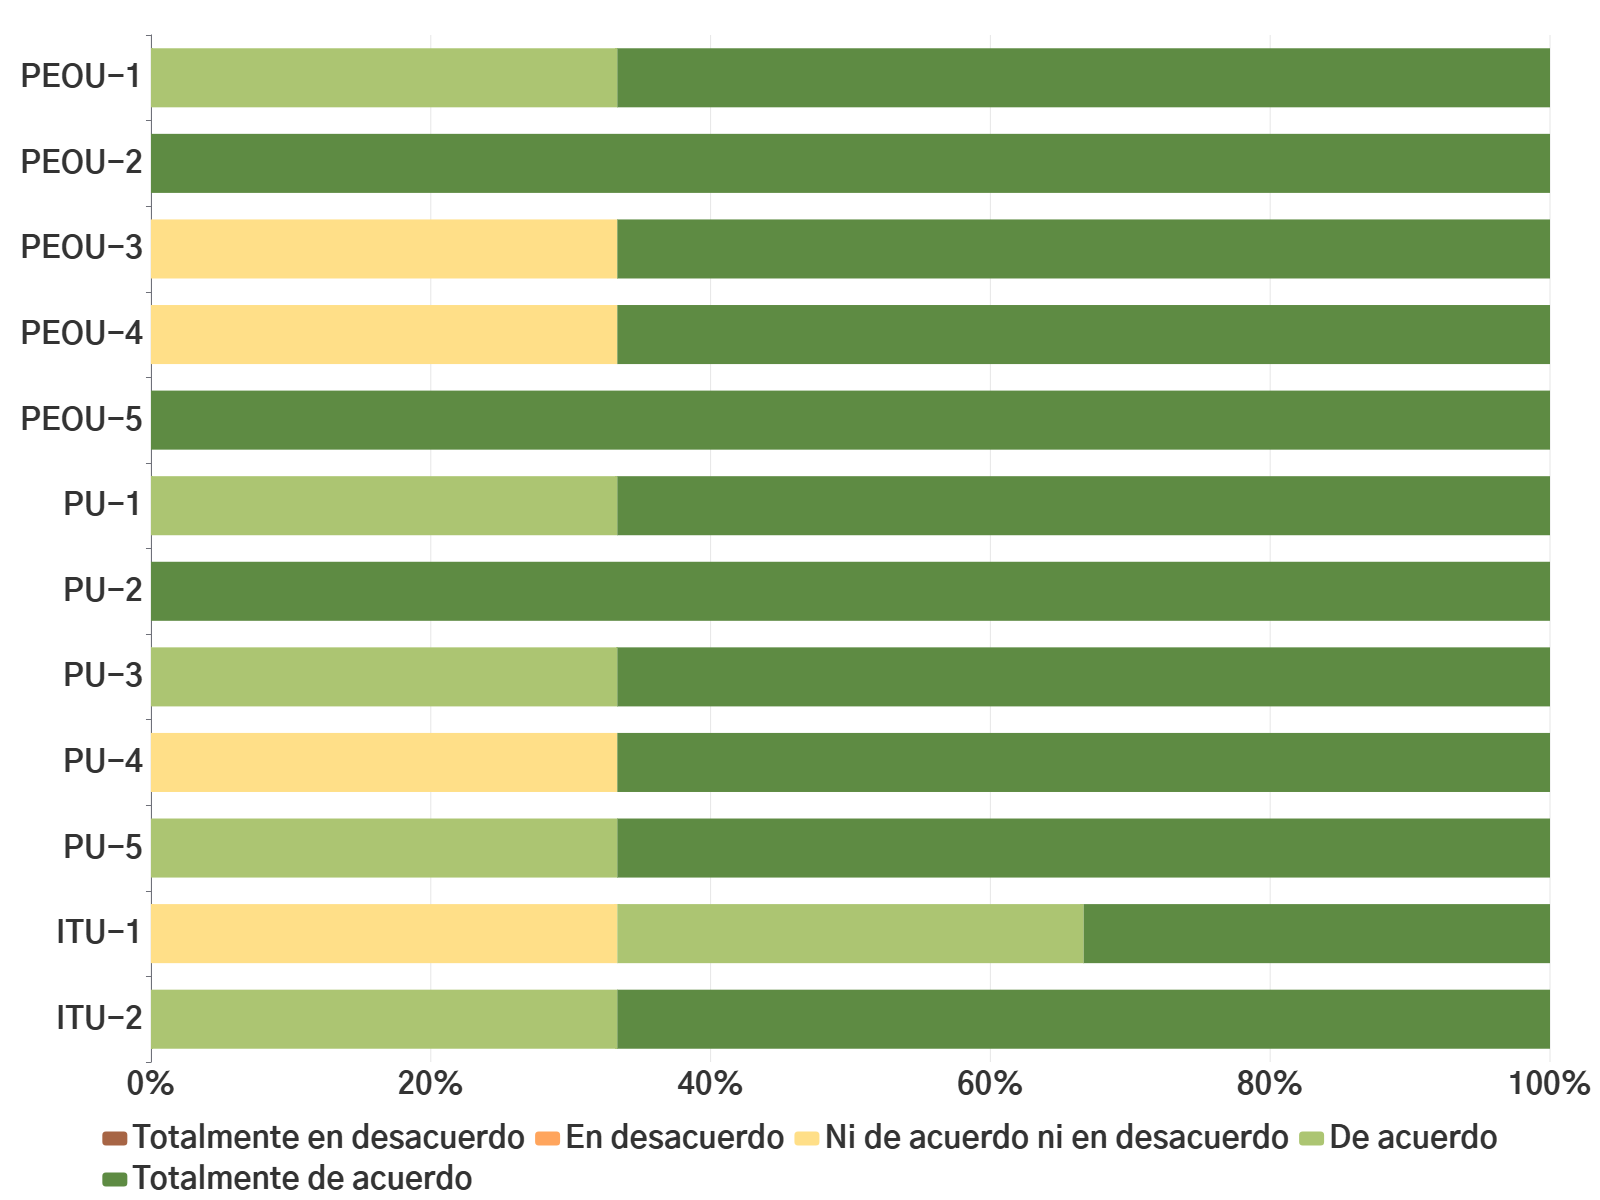
\includegraphics[width=1\textwidth]{tfgetsinf/images/GraficaEncuesta.png}
    \caption{Desglose de Resultados de la Encuesta}
    \label{fig:StackedChart}
\end{figure}

\subsection{Matriz de trazabilidad}

Para recopilar y consolidar los resultados de la validación se ha elaborado la matriz de trazabilidad a continuación. Esta tabla relaciona cada requisito clave del proyecto (funcional, no funcional y de aceptación) con el medio de validación empleado, el criterio de éxito encargado y el resultado final obtenido.

\renewcommand{\arraystretch}{1.4}
\begin{longtable}{|p{3.7cm}|p{3.7cm}|p{3.8cm}|>{\centering\arraybackslash}m{2cm}|}
    \hline
    \textbf{Elemento a Validar} & \textbf{Método de Validación} & \textbf{Criterio de Aceptación} & \textbf{Resultado} \\
    \hline
    \endfirsthead

    \multicolumn{3}{l}{\footnotesize Continues from previous page} \\
    \hline
    \textbf{Elemento a Validar} & \textbf{Método de Validación} & \textbf{Criterio de Aceptación} & \textbf{Resultado} \\
    \hline
    \endhead

    % --- PIE DE PÁGINA PARA TODAS LAS PÁGINAS MENOS LA ÚLTIMA ---
    \hline
    \multicolumn{3}{l}{\footnotesize Continues on the next page} \\
    \endfoot

    % --- PIE DE PÁGINA PARA LA ÚLTIMA PÁGINA ---
    \endlastfoot

    % --- CONTENIDO DE LA TABLA ---
    \multicolumn{4}{|c|}{\textbf{Historias de Usuario (Funcionalidad y Usabilidad)}} \\
    \hline
    HU01: Iniciar sesión & Observación directa & El 100\% de los usuarios completa el \textit{login} sin ayuda. & \cmark \\
    \hline
    HU02: Panel de control & Observación directa & El 100\% de los usuarios localiza el panel y entiende la información. & \cmark \\
    \hline
    HU03, HU05-07: Crear y configurar un análisis & Observación directa & El 100\% de los usuarios completa el formulario de creación y configuración sin errores críticos. & \cmark \\
    \hline
    HU04: Gestión de análisis & Observación directa & El 100\% de los usuarios es capaz de filtrar, ver detalles y eliminar un análisis. & \cmark \\
    \hline
    HU08: Ejecución del análisis & Observación directa & El 100\% de los usuarios inicia un análisis y verifica su estado \textit{running}. & \cmark \\
    \hline
    HU09: Visualización de resultados & Observación directa & El 100\% de los usuarios accede correctamente al informe de resultados. & \cmark \\
    \hline
    HU10: Exportación de resultados & Observación directa & El 100\% de los usuarios descarga con éxito el informe del análisis. & \cmark \\
    \hline
    HU11: Notificaciones & Inspección de correo y \textit{UI} & El sistema envía notificaciones por correo y en la app al finalizar un análisis. & \cmark \\
    \hline \hline
    \multicolumn{4}{|c|}{\textbf{Requisitos No Funcionales (Rendimiento y Seguridad)}} \\
    \hline
    RNF-001: Seguridad & Inspección técnica & Uso de \textit{HTTPS} y proveedor de identidad externo (\textit{Auth0}). & \cmark \\
    \hline
    RNF-002: Tiempo de carga & Medición directa & El tiempo de carga del panel de control es inferior a 2 segundos. & \cmark \\
    \hline
    RNF-003: Rendimiento \textit{Lighthouse} & Auditoría automatizada & La puntuación de rendimiento en \textit{Lighthouse} es $\geq$ 90. & \xmark \\
    \hline \hline 
    RNF-004: Interfaz intuitiva & Observación directa & El 100\% de los usuarios completa las tareas sin errores críticos. & \cmark \\
    \hline
    \multicolumn{4}{|c|}{\textbf{Modelo de Aceptación Tecnológica (\textit{TAM})}} \\
    \hline
    PEOU: Facilidad de Uso Percibida & Cuestionario \textit{TAM} & La puntuación media de los ítems PEOU es $\geq$ 4/5. & \cmark \\
    \hline
    PU: Utilidad Percibida & Cuestionario \textit{TAM} & La puntuación media de los ítems PU es $\geq$ 4/5. & \cmark \\
    \hline
    ITU: Intención de Uso & Cuestionario \textit{TAM} & La puntuación media de los ítems ITU es $\geq$ 4/5. & \cmark \\
    \hline
    
    \caption{Matriz de Trazabilidad de la Validación.}
    \label{tab:matriz_trazabilidad} 
\end{longtable}
\renewcommand{\arraystretch}{1.0} % Restaurar el valor por defecto

La validación integral de \textit{PhenoScore} ha proporcionado una evaluación completa de la plataforma, extrayendo resultados mayoritariamente positivos que confirman el éxito del proyecto en sus objetivos fundamentales.

El análisis funcional y de usabilidad ha demostrado que la plataforma es robusta y cumple eficazmente su propósito principal, ya que los tres perfiles de usuario completaron con éxito el 100\% de las tareas guiadas. Este resultado es la evidencia de que \textit{PhenoScore} logra reducir la barrera tecnológica, ofreciendo una interfaz intuitiva y accesible para un dominio que ha demostrado ser complejo.

La evaluación de los requisitos no funcionales ha verificado que la aplicación es segura y tiene un rendimiento óptimo en escenarios de uso individual, con tiempos de carga rápidos y con una base técnica sólida.

Finalmente, los resultados del Modelo de Aceptación Tecnológica (\textit{TAM}) refuerzan las observaciones positivas, concluyendo que los usuarios consideran la plataforma fácil de usar, además de percibirla como una herramienta de gran utilidad, estando dispuestos a integrarla en su flujo de trabajo profesional.

En conclusión, la validación confirma que \textit{PhenoScore} es una plataforma exitosa, una solución funcional, usable y bien valorada por los usuarios objetivo, con una línea clara de futuras mejoras en su escalabilidad.